%! Author = Ian's PC
%! Date = 9/13/2023

% Preamble
\documentclass[11pt]{article}

% Packages
\usepackage{amsmath}
\usepackage{graphics}
\usepackage{graphicx}
\usepackage{amsfonts}

\title{Assignment 2 Writeup}
\author{Ian Chen}
\date{\today}

% Document
\begin{document}
    \maketitle


    \section{Short answer problems}

    \begin{enumerate}
        \item \textit{Compare the effects of 1) Dilation + Erosion against 2) Erosion + Dilation. Do they have the same
        effects? Why?}\newline
        They have different effects. Erosion then dilation, also called opening, is used to
        remove small objects while preserving original shape. This effect removes small regions-like objects like lines
        or noise, while preserving the larger areas. Dilation then erosion, also called closing, fills holes in regions
        while preserving region sizes. This effect fills in gaps between objects or within the object itself, while
        preserving large holes and regions.\newline

        \item \textit{List two examples of regular texture and two examples of near-regular texture.}\newline
        Regular- Brick Wall and Checkerboard. Both are exact patterns and identical shapes with no randomness.\newline
        Irregular- Stone Floor Tiles and Wood Planks. Both are identical from far away, but when closely examined, have
        small details unique to each piece.\newline

        \item \textit{What are the cases where optical flow is not well-defined? Please give two concrete examples.}\newline
        One case is the aperture problem, where the object's motion is not aligned with the direction calculated by the
        optical flow gradient, such as a spinning barber pole, with the pixels seem to move up constantly, while in
        reality it's moving either clockwise or counter-clockwise. The occlusion of the object's motion causes a false
        interpretation of its motion.\newline
        Another case is the inconsistent brightness, where the object's brightness changes over time, such as a
        light source being moved around. The optical flow gradient will be inconsistent and not well-defined.\newline
        Another case is texture-less regions, where the object has no texture, such as a white wall. The optical flow
        gradient will not sense motion, since all pixels have the same brightness.\newline
        Another case is motion too fast for the frame rate, where the object moves too fast for the camera to capture
        smooth differences between each frame. This causes the optical flow gradient to be unable to track motion
        throughout the frames.\newline

        \item \textit{What are the advantages of RANSAC when compared with Hough Transform?}\newline
        RANSAC is more robust to outliers than Hough Transform. RANSAC is able to detect and identity more types of
        shapes than Hough, so it's more applicable to a wider variety of images. RANSAC is also more efficient than
        Hough Transform, since only a subset of the total points are needed to be sampled to have a confident result
        that's representative of the entire image.\newline

    \end{enumerate}


    \section{Circle Detection}

    Implement two circle detectors (one based on Hough Transformation and another based on RANSAC) that takes an input
    image and a fixed (known) radius, and returns the centers of any detected circles of about that size.
    Include two functions with the following form:
    \begin{center}
    [centers]
        = detectCirclesHT(im, radius)
    \end{center}
    \begin{center}
    [centers]
        = detectCirclesRANSAC(im, radius)
    \end{center}
    where ‘im‘ is the input image, ‘radius‘ specifies the size of circle we are looking for.
    Your detector should not exploit the gradient direction. The output centers is an N x 2 matrix in which each row
    lists the x,y position of a detected circle’s center. Write whatever helper functions are useful. Then experiment
    with the basic framework, and in your writeup analyze the following:

    \begin{itemize}
        \item \textit{Explain your implementation in concise steps (English, not code).}\newline
        I first found the edges of the image using the Canny edge detector. Then, I created an accumulator
        array filled with all zeroes. Then, I looped through the edges and incremented the accumular values of the
        matrix if the center was an edge pixel. Then, I found the maximum value of the accumulator array and
        determined that it was the center of the circle.\newline

        \item \textit{Demonstrate the functions applied to the provided images ‘coins.jpg‘ and ‘planets.jpg‘ and one
        image of your choosing. Display the images with detected circle(s), labeling the figure with the radius.
        Note: you only need to select one reasonable radius and display all detected circles
            (i.e., those with highest votes) under that radius.
            You are not required to consider circles with a center off the image.}\newline
        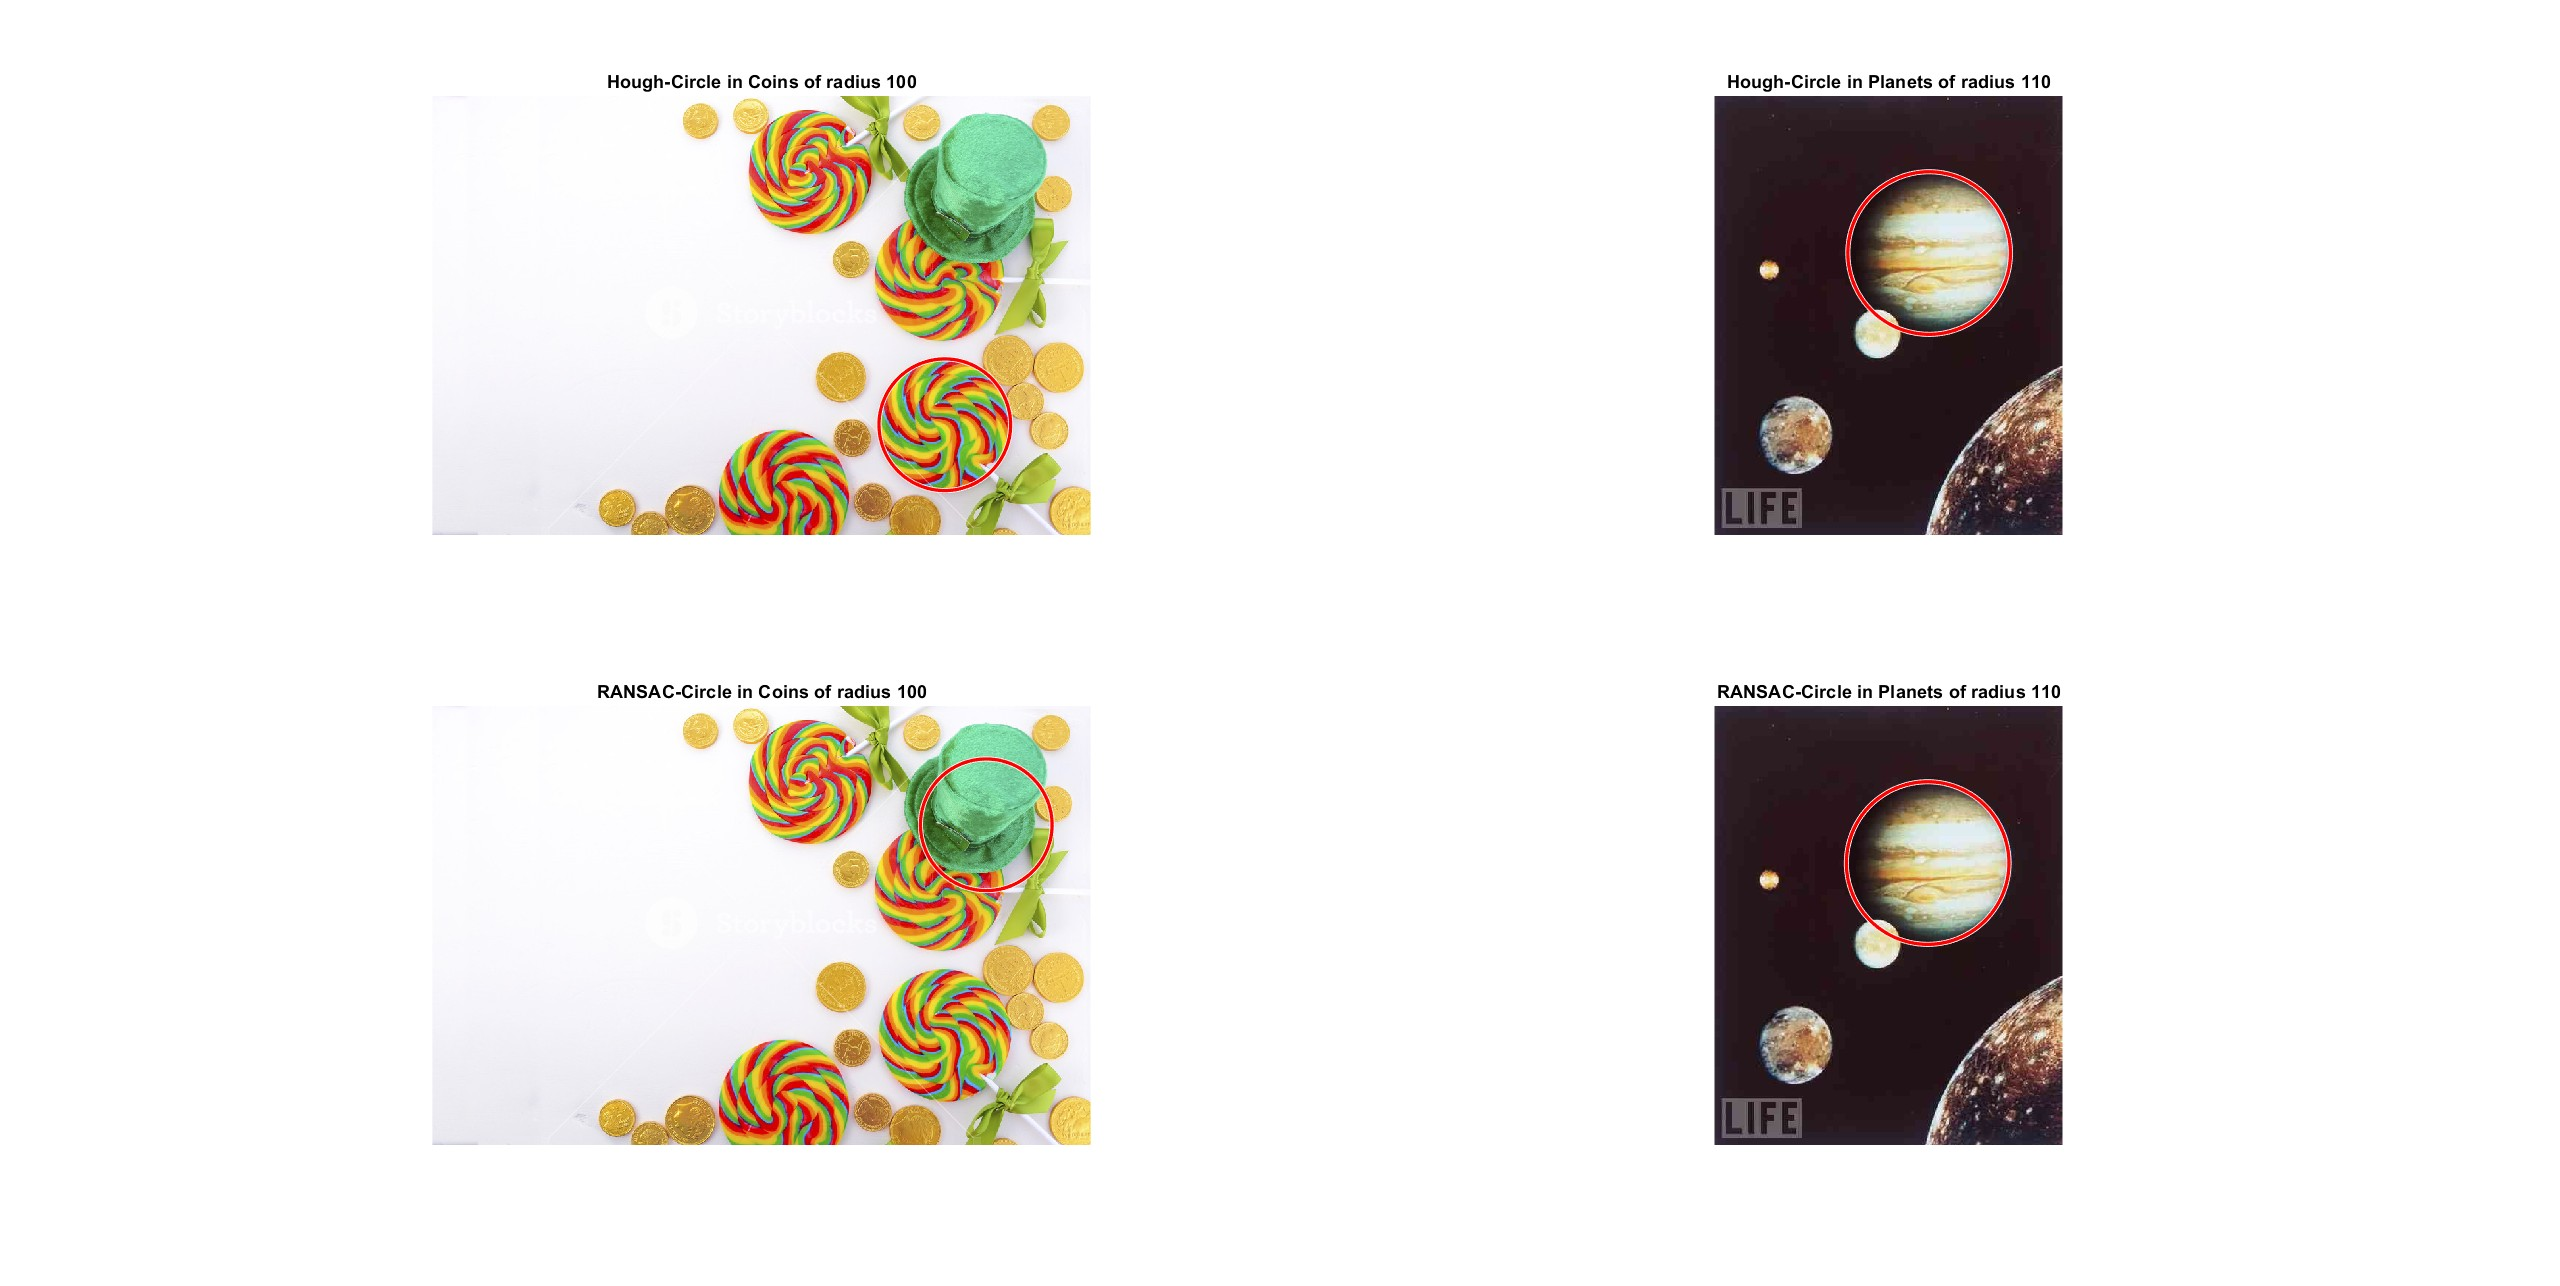
\includegraphics[width=\textwidth]{Output Pictures/detection_output}\newline

        \item \textit{For Hough Transform, explain how your implementation post-processes the
        accumulator array to determine automatically how many circles are present.}\newline
        I first got the local maximums of the accumulator array and zeroed out all values not at a local max. This
        removes circle overlap of thick edges. Next, I used a constant threshold of 120, which means one-third of the
        circle's edge touches this point. This is to account for noise and a circle not being perfectly round. This
        removes detected circles overlapping due to only the local maximums being considered. Therefore, all local
        maxima with 120 edge points going through them are considered circles.\newline

        \item \textit{For RANSAC, explain how you implement circle fitting.}\newline
        I first randomly selected three points from the edge points. Then, I calculated the center and radius of the
        circle based on those three points. If the radius was within a threshold of the expected radius, then it was
        a potential fit. Then, I used a threshold to determine how many edge points were within that threshold from
        the calculated radius, if enough points were within, based on the statistical equation:
        $\mathbb{N}$ = $\frac{\log(1 - p)}{\log(1 - w^n)}$.\newline

        \item \textit{For one of the images, display and briefly comment on the Hough space accumulator array.}\newline
        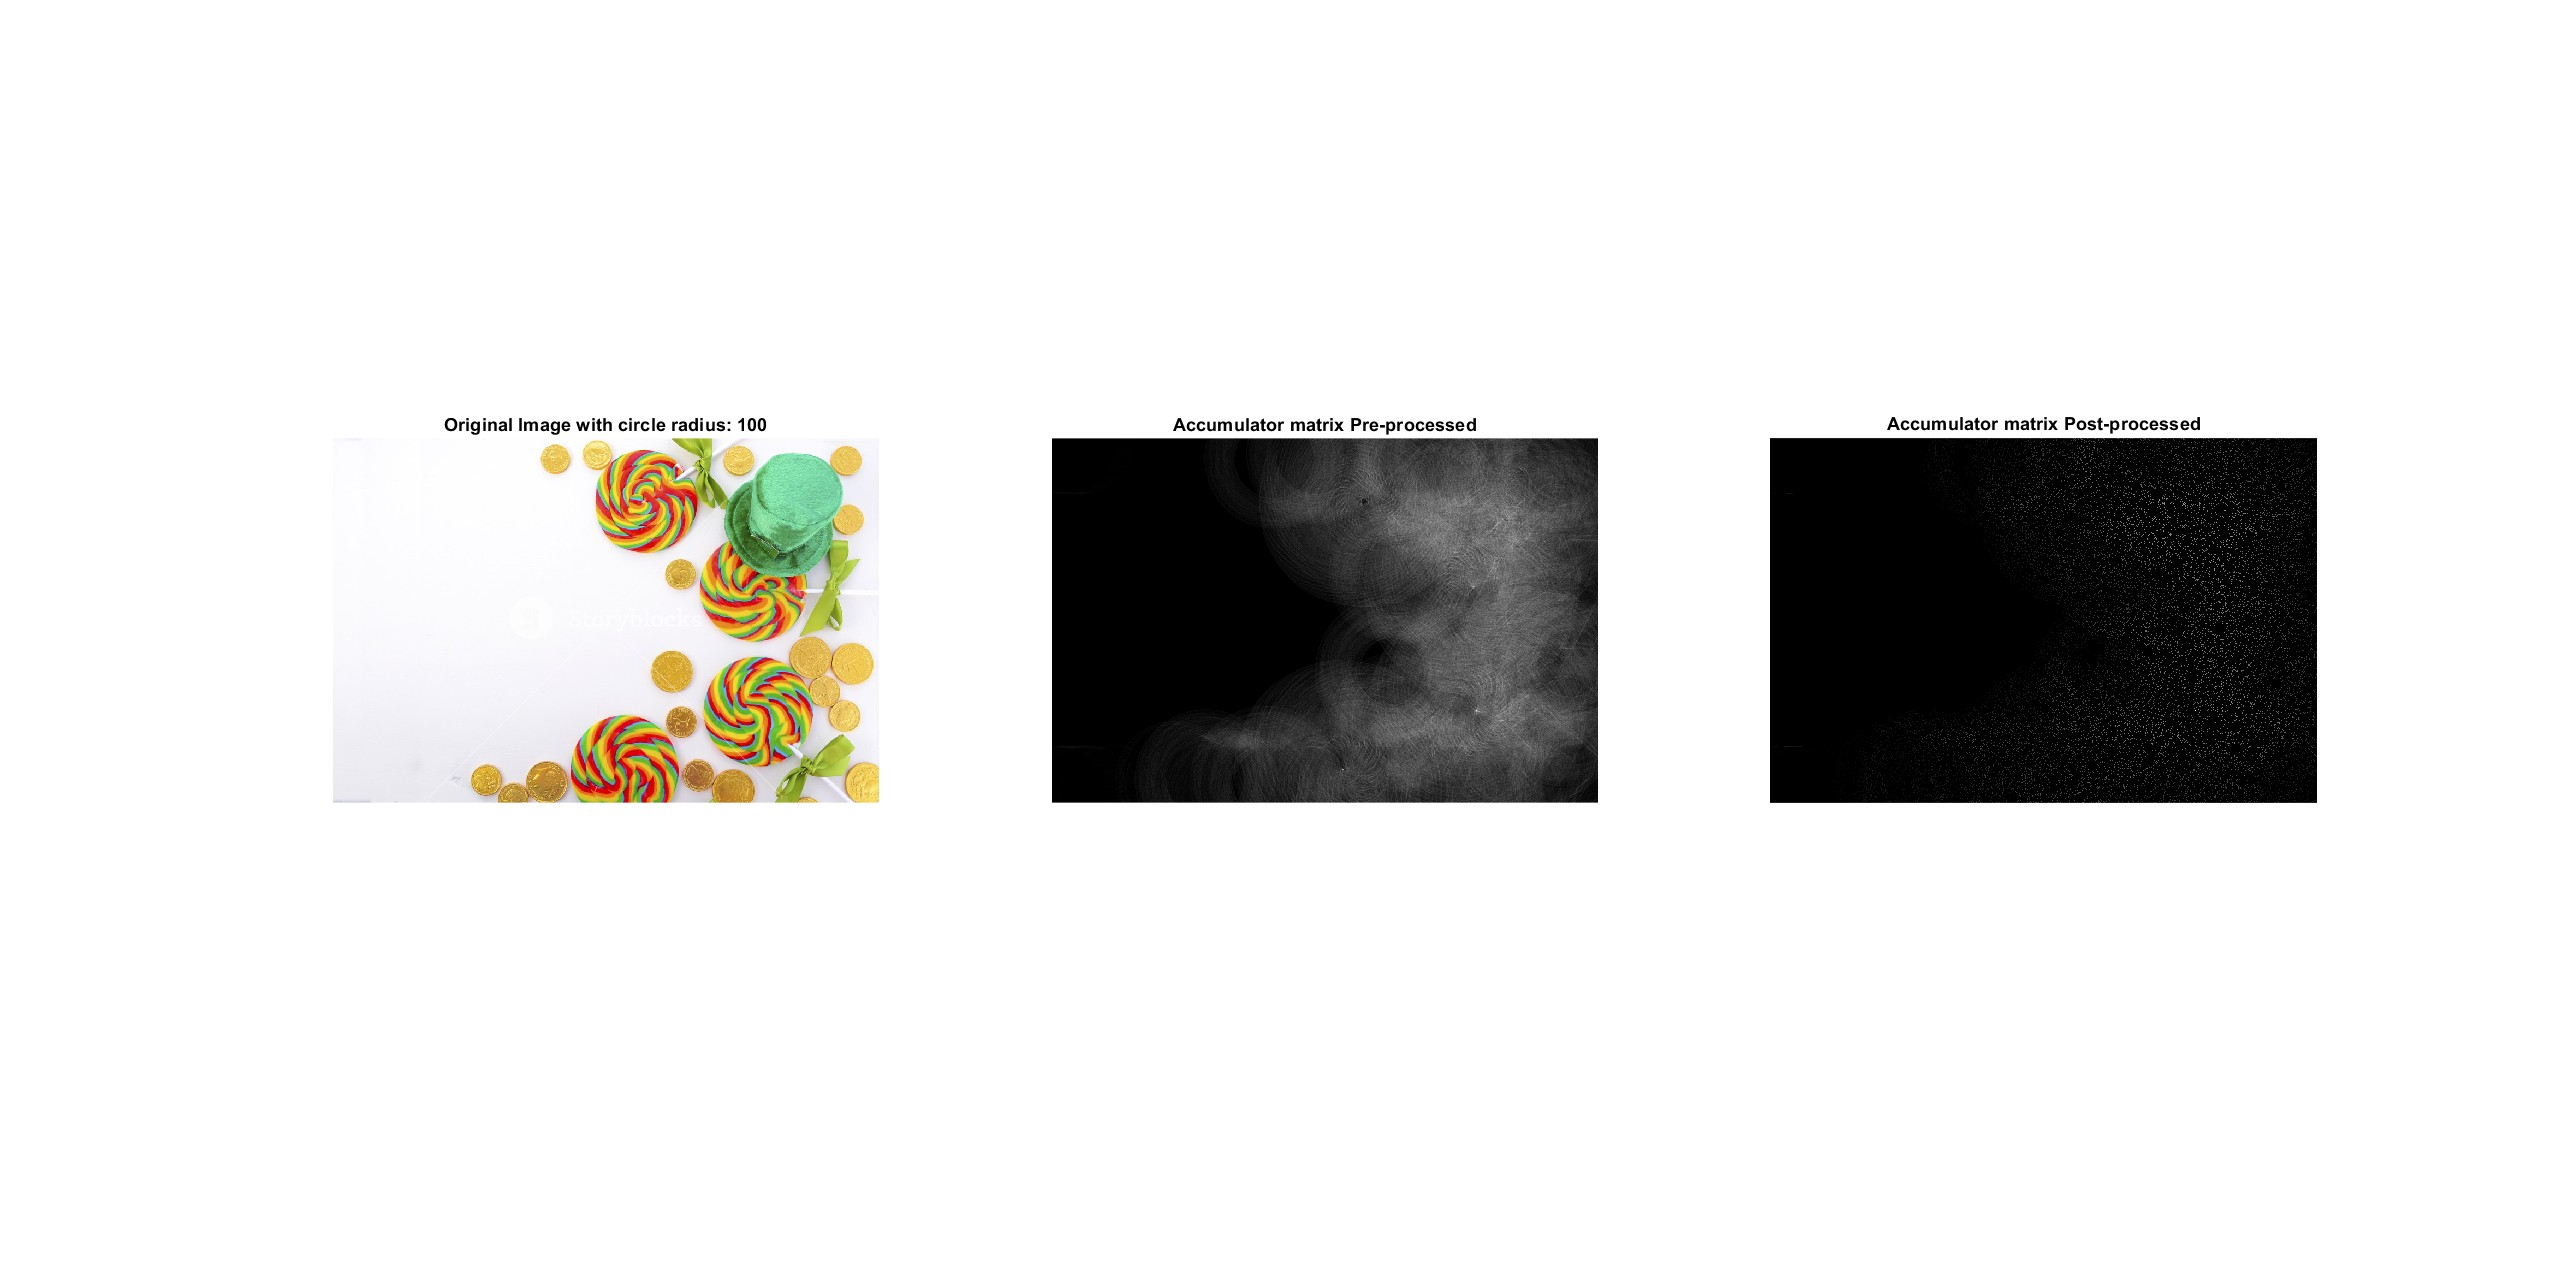
\includegraphics[width=\textwidth]{Output Pictures/hough_accumulator}\newline

        \item \textit{For one of the images, demonstrate and explain the impact of the vote space quantization (bin
        size). In other words, alter the bin size and compare and contrast with a brief explanation why/what happened
        makes sense.}\newline
        Smaller bin sizes result in a more finely quantized accumulator array. This can lead to higher sensitivity
        which may produce more noise and false positives. Circles with radii close to the expected radii will be
        detected, but it may miss some circles with slightly different radii due to the quantization effect.
        Larger bin sizes result in a coarser quantization of the accumulator array. This can reduce sensitivity but
        may miss partially occluded circles. It may be more robust against noise but may miss small or slightly
        distorted circles.\newline
        The choice of the bin size is a fine balance between sensitivity and noise tolerance, depending on the specific
        application and the expected properties of the circles in the image.
        Smaller bin sizes are suitable for high-precision applications,
        while larger bin sizes may be preferred in noisy or less structured images.\newline

        \item \textit{For one of the images, plot the progress of the RANSAC as the number of tries increase. The x axis
        of the plot should be the number of tries, and the y axis should be the number of inliers that the best model
        produces.}\newline
        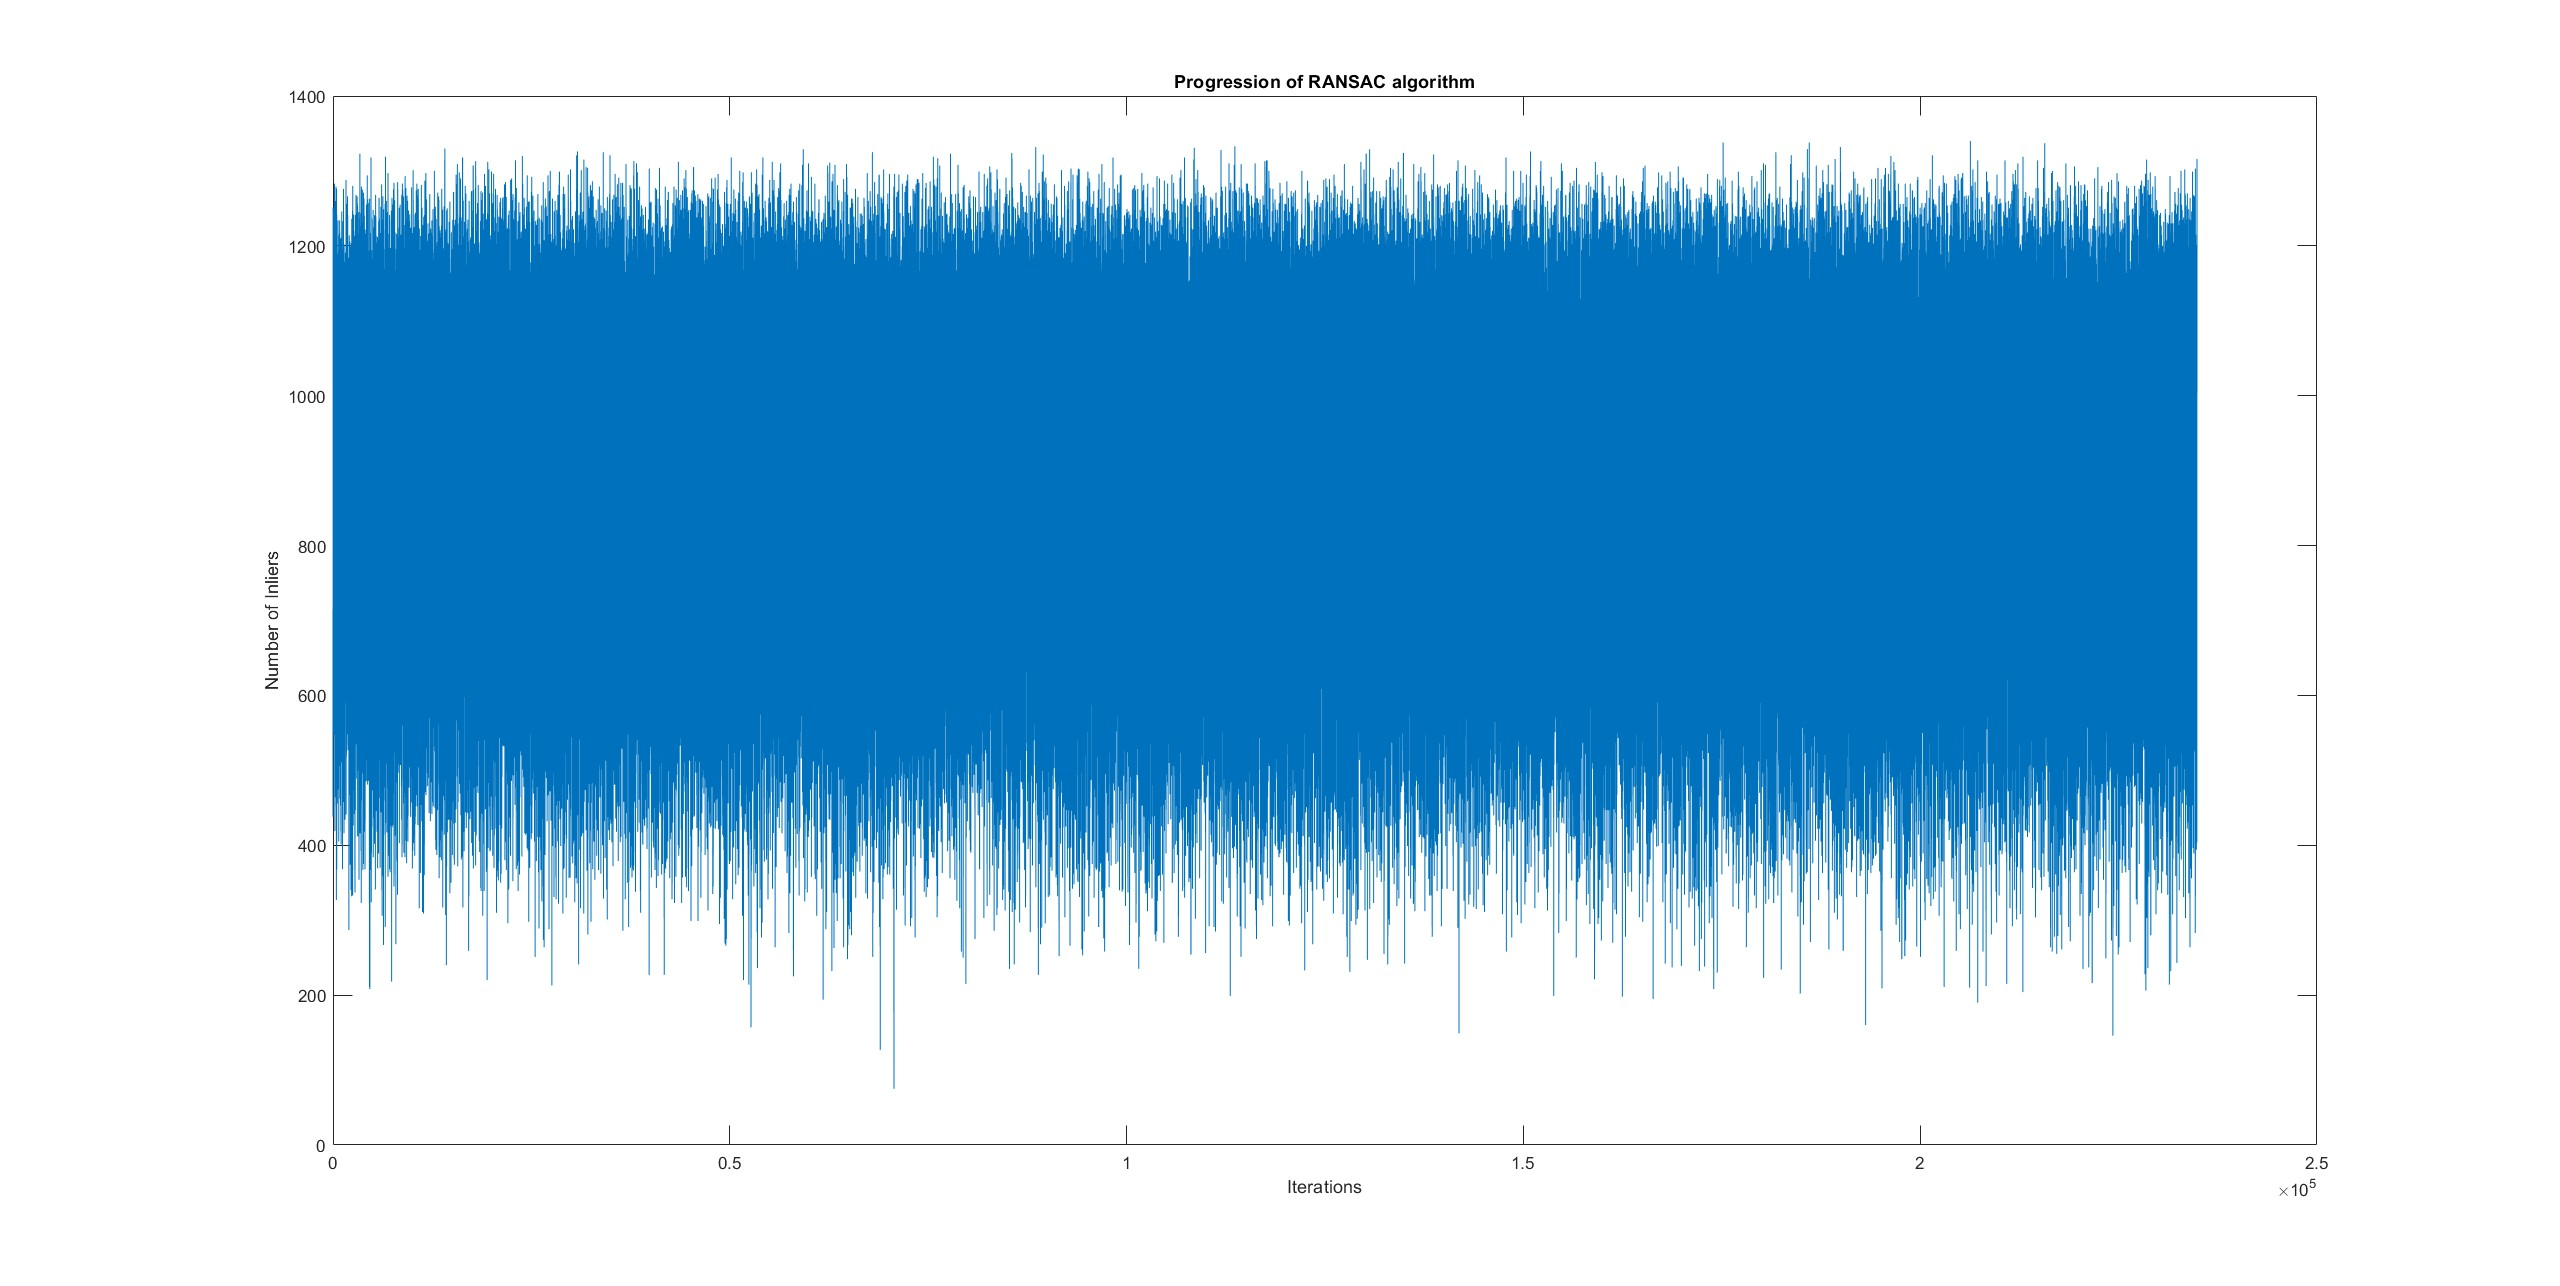
\includegraphics[width=\textwidth]{Output Pictures/inlier_progression}\newline

    \end{itemize}


    \section{Image segmentation with k-means}

    \begin{enumerate}
        \item \textit{Given an h x w x 3 matrix ‘Im‘, where h and w are the height and width of the image, apply
        k-means clustering to
        associate pixels with clusters. Return ‘labelIm‘, an h×w matrix of integers indicating the cluster
        membership (e.g., from 1 to k) for each pixel.
        Please use the following form:}\newline
        \begin{center}
            function [labelIm] = clusterPixels(Im, k)
        \end{center}

        \item \textit{Detect cluster boundary pixels from ‘labelIm‘.}\newline
        \begin{center}
            function [boundaryIm] = boundaryPixels(labelIm)
        \end{center}

        \item \textit{Please test both functions on the provided images ‘gumballs.jpg‘, ‘snake.jpg‘, and ‘twins.jpg‘
        and one other image of your choosing, and then displays the results.}\newline

    \end{enumerate}
\end{document}